\documentclass{acm_proc_article-sp}

%encoding
%--------------------------------------
\usepackage[utf8]{inputenc}
\usepackage[T1]{fontenc}
\usepackage{pgfplots}

%--------------------------------------
 
%Portuguese-specific commands
%--------------------------------------
\usepackage[portuguese]{babel}
%--------------------------------------
 
%Hyphenation rules
%--------------------------------------
\usepackage{hyphenat}
\hyphenation{mate-mática recu-perar}
%--------------------------------------
\usepackage{graphicx}
\usepackage{placeins}
\usepackage{balance}
\usepackage{color,graphicx}


\begin{document}

\title{A Tool for Automated Testing of the HEVC Video Encoder}


\numberofauthors{6}
\author{
\alignauthor
José Raimundo Barbosa\\
       \affaddr{Grupo de Processamento Digital de Sinais (GPDS)}\\
       \affaddr{Instituto Federal da  Paraíba}\\
       \email{j.zmais@gmail.com}
\alignauthor
Carlos Danilo Miranda Regis\\
       \affaddr{Grupo de Processamento Digital de Sinais (GPDS)}\\
       \affaddr{Instituto Federal da  Paraíba}\\
       \email{regis.danilo@gmail.com}
\alignauthor
Ruan Delgado Gomes\\
       \affaddr{Laboratório de Computação Embarcada e Distribuída (Laced)}\\
       \affaddr{Instituto Federal da  Paraíba}\\
       \email{ruandgomes@gmail.com}
\and % go to new row
\alignauthor
Jean Felipe Fonseca de Oliveira\\
       \affaddr{Instituto de Estudos Avançados em Comunicações (IECOM)}\\
       \email{jeanfelipefonseca@gmail.com}
}
\maketitle
\begin{abstract}

H.265/HEVC is the state-of-the-art video codec, focusing in Ultra-High Definition video (UHD) and it is 50\% more efficient in bit-rate compression than its predecessor, the H.264/AVC. However this efficiency requires a high computational cost, which may compromise the use of the encoder in limited machines or in real time applications that use UHD videos. Several studies look for ways to enhance the HEVC encoder and reduce the computational cost. However, to develop optimized versions of the encoder it is necessary to perform tests that can last for hours and usually requires manual collection of coding information.  In this work, a tool to perform automated tests of HEVC encoders  was developed. The tool was implemented in a parallel architecture that allows the execution of several instances of the encoder. It collect the informations and executes objective metrics to evaluate the efficiency of the encoder, the dualty of the encoder video and the encoding time. \textcolor{blue}{This work intends to provide a useful solution to help analyze encoders in long sequences of tests}.

\end{abstract}

\keywords{Automated testing, HEVC encoder, UHD videos} 

\section{Introduction}

Currently, about three-quarters of annual data traffic on the Internet is assigned to video content, according to Cisco's Visual Networking Index report. In 2014 this consumption was 64\% and in 2020 this value will be about 80\%~\cite{Cisco:16}. One of the contributing factors is the increase in video quality, which makes it possible to explore more and more new experiences on Internet-broadcast television channels, video conferencing and on-demand video transmission services such as YouTube and Netflix, which Already distribute videos in UHD~\cite{cheon:14}.

The UHD videos are highly popular in the market, because high pixel density makes it possible to increase the perception of image details, allowing new experiences for viewers~\cite{cheon:14}. UHD 4K videos, for example, have resolution of 4096x2160 pixels while previous standards such as Full HD have 1920x1080. However, a UHD 4K stream raw, with 24 bits per pixel and 24 frames per second, requires a bandwidth of 5 Gbit/s~\cite{gomes:13}. These settings represent challenges in to storage and transmission of such videos.

To enable the intense and growing traffic of videos on the Internet and to satisfy the bandwidth conditions about the UHD characteristics, it is necessary to develop codecs responsible for digital video signal compression and descompreesion, which reduces the storage space and adjusts data volume to bandwidth limitations~\cite{oliveira:16}\cite{wang:13}. However, when compression occurs several times or in the wrong way, it generates loss of information that can degrade image quality~\cite{netflix:16}. In this context, the challenge arises of developing codecs capable of meeting the demand for UHD videos, and maintaining compression efficiency and image quality.

The ITU-T H.265~\cite{itu:265}, also known as High Efficiency Video Coding (HEVC), is the state-of-the-art codec which focus primarily on new UHD video technologies and presents a compression efficiency 50\% higher than its predecessor. H.264/Advanced Video Coding (AVC)~\cite{Bossen:12}\cite{Hanhart:12}\cite{Sullivan:12}. However, the HEVC has a computational cost up to four times higher than H.264. This is attributed to the processing of the new block structures used in the compression, which increases the computational cost presents challenges for situations that demand real-time video reproduction or in machines with processing limitations~\cite{Yoon:13}\cite{Correa:12}.


To promote HEVC optimization research, JVC-TV provided the HM reference encoder which features a basic implementation of HEVC that makes possible  to carry out studies on the efficiency of the codec and develop new features and optimizations~\cite{itu:10}. However, evaluating codecs developed based on the HM reference source code is a normally time-consuming process, since each test implies in the execution of several instances of the evaluated codec and the reference codec, which can last for several hours. After execution, is necessary to compare the UHD videos using objective or subjective metrics. With the comparisons it is possible to monitor the efficiency and performance of the new encoders compared to stable versions in the UHD scenario~\cite{netflix:16}.

This paper describes a tool for automated testing of HM based encoders. The tool was implemented in a parallel architecture in which multiple instances of the encoder are executed simultaneously. To calculate the encoder efficiency and the difference between the codecs the Bjontegaard metric is used, this metric determines the difference of the efficiency of the codecs from the calculation of the mean difference of two curves adjusted by four points~\cite{Bjontegaard:01}, For the formulation of the standardized test cases, the recommendations of JCT-VC were followed~\cite{Bossen:15}. With the tool the comparison between the~\cite{oliveira:16} codec and reference codec~\cite{itu:10} was obtained and reduction of the test time by 86\% in a simple test case was verified, in which one video and one configuration were used, totaling the execution of 8 instances.
	
	
\section{Proposed test scenario}
	
%\subsection{Reference Codec HM}



The Joint Collaborative Team on Video Coding (JCT-VC) provided a open source HM reference encoder, which offers a basic implementation of HEVC in C++~\cite{Bossen:15}.The HM code provides an environment for the development of new features or optimizations, such as those developed in~\cite{oliveira:16}\cite{Yoon:13}\cite{Correa:12}\cite{Weerakkody:14}. In conjunction with the encoder, JCT-VC also provides the recommended settings and videos for standardized test suites. These settings will be presented later.

After encoding, HM generates, in addition to the encoded video, a record file in which important information about the encoding process is present such as bit rate, total encoding time, output video file size, PSNR for each YUV color matrix (Y = Luma, U = Chroma Blue and V = Chroma Red).

\textcolor{red}{
The way the tool was developed also makes it possible to perform tests with the Joint Exploration Model (JEM) reference encoder~\cite{Bossen:17}. This encoder was developed based on HM and was presented in~\cite{JVET:2015} as the future of the environment for standardized development of HEVC video compression technology, including its current extensions and near-term extensions for screen content coding and high-dynamic-range coding.
}


\subsection{Standardization of Tests}

To ensure common testing conditions, the JCT-VC committee has developed the JCTVC-L1100 documentation \cite{Bossen:13}, which describes the settings and contents for standardized tests that explore different situations. This standardization is applied in the development of new features or encoder optimizations developed using HM. The settings discussed in the document are:

\begin{itemize}

  \item All Intra: All frames are encoded independently with only intra-frame prediction.
  \item Random Access (RA): Coding with high rates of compression compression. The coding order and the output order of the frames differ, inducing a coding delay. This setting represents broadcast and streaming applications.
  \item Low Delay P (LP): Coding without the structural coding delay presented when using RA parameters. This configuration is evaluated using only P-frames (uni-directional prediction).
  \item Low Delay B (LB): Similar to LP scenarios, but this configuration is evaluated using only B-frames, (unidirectional and bidirectional prediction).

\end{itemize}

These settings specify situations with videos with 8 bits of depth, besides these there are also the configurations directed to videos with 10 bits. In the documentation, the videos present in \emph{ftp://hevc@ftp.tnt.uni-hannover.de/testsequences/} are also recommended, requiring a registration to access the videos. Finally, the quantization values are specified: 22, 27, 32 and 37. In the tool, these values are already configured with standards, but it is possible to add more quantization values.


\subsection{Bjontegaard Metric}

The Bjontegaard metric is considered state-of-the-art in relation to the evaluation of video coding mechanisms and is one of the most widespread in the current literature~\cite{Bjontegaard:01}\cite{Mathias}. This allows to obtain the values for overall bit rate (BD-Rate) in percent for two different encoding algorithms
considering the same PSNR or overall video quality difference (BD-PSNR) for two different encoding algorithms considering the same bit rate. %These values are used to evaluate the efficiency of the modified encoders in relation to the HM reference encoder.
	
The BD-PSNR is the measure corresponding to the average difference of Peak Signal-to-Night Ratio (PSNR) in decibels, between two encoders, considering the same bit rate. While the BD-Rate value corresponds to the average percentage bit difference for the two encoders. In this work, more attention was given to bit rate evaluation.	

\textcolor{red}{
In \cite{Mathias}, exemplifies the BD-Rate by means of Figure \ref{fig:chart_barate}, where the curves are further drawn by linear interpolation. For the BD calculations, the rate axis is logarithmized and the rate-distortion curves are interpolated by an advanced interpolation method. The overlapping portions of the rate-distortion curves are used for calculation of the BD values. The BD-rate, the difference in horizontal direction. Depending on the range of overlap of the two curves, the resulting BD measurements get more or less meaningful. Therefore, careful interpretation of the resulting numbers is required.
}

\FloatBarrier
\begin{figure}[!ht]
	\centering
	\caption{Interpolation of the BD-Rate \cite{Mathias}}
	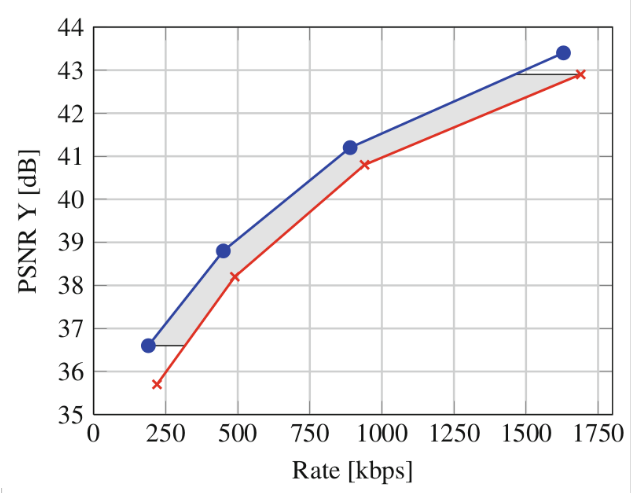
\includegraphics[width=0.4\textwidth]{figures/chartbdrate.png}
	\label{fig:chart_barate}
\end{figure}
\FloatBarrier
	
%\Delta R = \frac{R_{B}(D) - R_{A}(D)}{R_{A}(D)}

%\Delta R = 10^{r_{B}{(D)}-r_{B}{(D)}}-1

%SI = \left ( \frac{1}{N-1}\sum_{i=1}^{1}(\upsilon_{S}-S)^{2} \right )^{\frac{1}{2}}

%\begin{math}
%	\centering
%	\label{fig:bj}
%	PWSSIM(f,h)= \frac{\sum_{d=1}^{D}SSIM_{d}(f,h)*SI_{d}}{\sum_{d=1}^{D}=1^{SI_{d}}}		
%\end{math}

\section{Related Works}

	
	
\section{Tool Description}

To verify the efficiency it is necessary to perform several tests in which the modified encoder is executed in several coding scenarios, and then the results of each coding are compared with the results of the reference encoder. Each test sequence of an encoder can 
last for hours, depending on the videos and test settings, which hinders the development stage. The comparison is made between values such as bit rate, PSNR, coding time, and so on. These values are generated automatically by the HM encoder and are saved in log files. However, 
for their use it is necessary to manually collect in each log file so that it can be a repetitive work and result in errors from human failure. 

The tool developed in this work executes instances of the modified encoder and reference encoder in all required configurations and then automatically collects all the information necessary for the comparison. With the data collected from the log files the calculation of 
the Bjontegaard \cite{Bjontegaard} metric is performed, the tool architecture can be viewed in Figure \ref{fig:fluxo}. The modular way the tool was implemented enables other metrics to make use of the encoding values. To reduce the time of the tests, the tool was implemented in a parallel architecture in which multiple instances of the encoder are executed simultaneously, thus considerably reducing the time of a test.

\FloatBarrier
\begin{figure}[!ht]
	\centering
	\caption{Tool architecture}
	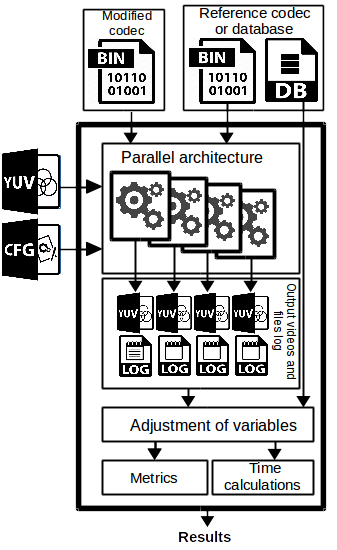
\includegraphics[width=0.4\textwidth]{figures/fluxo.png}
	\label{fig:fluxo}	
\end{figure}
\FloatBarrier

To prevent data loss during an unexpectedly stopped execution, a tool log file is generated that saves the current state of the test and makes it possible to return from where it left off. It is also possible to save the data of the tests performed by the encoders, thus avoiding to repeat the process and thus to promote the construction of a database with the results of the tests.

To execute the tests, the tool receives the parameters specified in Table \ref{parameter_tool}, these parameters indicate the settings that will be addressed equally by the modified encoder and the reference encoder that will generate different outputs. If not inform the parameters, default values will be used that will execute the tool used a CIF video (352x288) and a random configuration. 
These parameters have minimum specifications only for checking the operation of the tool. It is important to check the memory and thread limitations before running the tool, it is recommended to run one thread for every two GBs of RAM. In case of an unexpected interruption, the execution of the tool with the -bkp flag activates the backup and the test will return to the moment of interruption.

\FloatBarrier

\begin{table}[!ht]
%\vspace{-4in} 
\centering
\caption{Parameters for tool execution}
\label{parameter_tool}
\begin{tabular}{|l|l|p{3cm}|l|}
\hline
\textbf{Command} & \textbf{Example}      & \textbf{Description}                                         \\ \hline
./CodecTest      & --                    & Tool executable                                                             \\ \hline
-thr             & 2                     & Number of threads                                            \\ \hline
-vin             & 1 path/video.yuv  & Number of video followed by the video files                  \\ \hline
-cfg             & 1 path/File.cfg & Number of configuration followed by the configurations files \\ \hline
-outl            & path/out/logs/      & Path where log files will go                                 \\ \hline
-outv            & path/outvideos/    & Path where encoded videos will go                            \\ \hline
-eva             & path/BinEncoder    & Rated encoder binary                                         \\ \hline
-ref             & path/BinEncoder    & Reference encoder binary                                     \\ \hline
-fr              & 30                    & Frame rate                                                   \\ \hline
-f               & 130                   & Number of frames                                             \\ \hline
-q             	 & 4 22 27 32 37        & Number of quantization followed by the quantization values   \\ 
\hline
-wdt             & 3840                  & Video width                                                  \\ \hline
-hgt             & 2160                  & Video height                                                 \\ \hline
-bkp             & --                    & Backup flag                                                  \\ \hline
\end{tabular}
\end{table}
\FloatBarrier

The output file structure of the testing tool presents the key information about the execution of each instance, in addition to the total time values and the values of the metrics. A log file example is shown in Figure \ref{fig:log}.

\FloatBarrier

\begin{figure}[!ht]
	\centering
	\caption{File log example}
	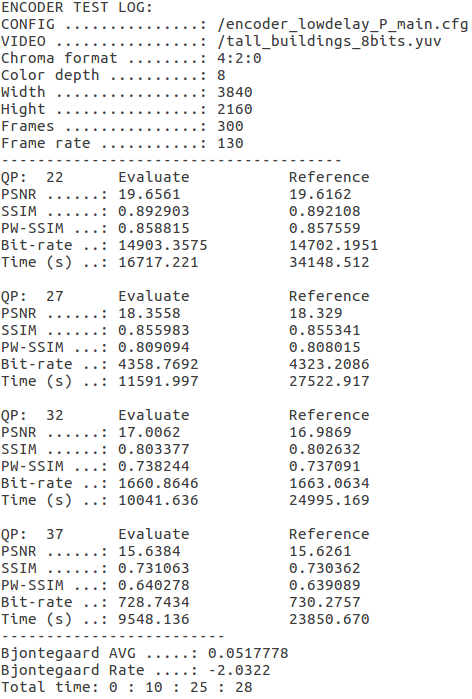
\includegraphics[width=0.4\textwidth]{figures/log.png}
	\label{fig:log}
\end{figure}

\FloatBarrier

For more complex tests, the implementation of a distributed version of the tool is in progress, which will allow the execution of more instances of the encoder according to the configuration and quantity available machines. Online services are also developed, in which researchers and developers can submit the executable program of their encoders and the configurations so that the tests are performed on a robust server. With this proposal also intends to build a database fed with the data of the tests of the users, this database will contribute to other researchers.
%---------------------------------------------------------	
	

%\pagebreak

\section{Result}

%- Acho que devemos ter uma seção para mais detalhes da Bjontegaard. E tem que deixar claro qual das métricas de Bjontegaard está sendo usada. BD-Rate nesse caso.
%- Precisamos melhorar o título, mas vamos deixar isso para depois

%- Na introdução é bom citar que o novo padrão já está sendo especificado e vários experimentos estão em testes. Ambientes como esse seriam bem propícios para o uso da ferramenta.

%- Os principais sistemas de transmissão de vídeo, seja transmissão terrestre ou internet streaming tem tendido a usar conteúdo em UHD, assim como mídeas de realidade virtual também terão resoluções "beyond-4K"

%- Vamos tentar caracterizar os testes Random Access, Low Delay P e Low Delay B. Vou procurar uma boa definição desses termos.

\bibliographystyle{waslon}
\bibliography{sample}


%\balancecolumns 

\end{document}